\documentclass[a4paper,12pt]{article}
\setlength\textwidth{7in}
\usepackage{amssymb,amsmath}
\usepackage{verbatim,graphicx}
\usepackage{fullpage}
\begin{document}

	\begin{titlepage}
		
		\vspace*{2cm}
		\begin{center}
		\large{\textbf{Comparison of Intrusion Detection Systems based on Machine Learning and Data Mining Algorithms for Low-Powered Devices}}
		\end{center}
		\vspace{0.5cm}
		\begin{center}
		\small{\textit{Project synopsis submitted} \\ \vspace{0.25cm} \textit{to} \\ \vspace{0.25cm}\textbf{MANIPAL ACADEMY OF HIGHER EDUCATION} \\}
		\end{center}
		\vspace{0.25cm}
		\begin{center}
		\small{\textit{For Partial Fulfillment of the Requirement for the\\ \vspace{0.25cm}Award of the Degree\\ \vspace{0.25cm}of}} \\ \vspace{0.25cm}
		\textbf{Bachelor of Technology} \\  \vspace{0.25cm} \textit{in} \\ \textbf{Computer and Communication Engineering}
		\end{center}
		\begin{center}
		\small{\textit{by}} \\
		\textbf{Pratyay Amrit} \\ \textbf{Reg. No. 140953430} \\
		\end{center}

		\begin{center}
		\small{\textit{Under the guidance of}} \\
		\renewcommand{\baselinestretch}{1}
		\vspace{0.5cm}
		Ms. Ipsita Upasana \\
		Assistant Professor \\
		Department of I \& CT \\
		 Manipal Institute of Technology \\
		Manipal, India 
		\end{center}

		\begin{figure}[h]
	  	\begin{center}
		
\includegraphics{MITLogo}
		\end{center}
		\end{figure}
		\begin{center}
		\textbf{Jan 2018}
		\end{center}

	\end{titlepage}

	%\newpage

	\newpage
	
	\section{Introduction}
	\paragraph{}
	Security in low-powered devices has always been a major concern as their limited computational capacity prohibits the use of sophisticated algorithms. An Intrusion Detection System(IDS) provides a first-line monitoring service for the devices to help them protect themselves against anomalous data. Several methods have been proposed to implement such a system. This work attempts to analyze and compare the performance of some of these methods under similar scenarios. the KDD'99 data-set is used to implement and compare these systems. 
	
	\section{Problem Definition}	
	\paragraph{}
	Technology is growing rapidly every day, and so are incidents concerned with cyber security. Intrusion Detection Systems are responsible for monitoring the network and detecting a data packet that may pose a risk for the network. Primitive IDSs were built to detect attacks on the basis of their signature. Every time a new attack was discovered, it's signature was recorded to protect the system from similar future attacks. This, however, could not prevent the system from new attacks. With the advent of Machine Learning and Data Mining techniques, these IDSs could now be taught how an attack looks in the network to perform detection of new attacks. This however, significantly increased the false positives in detection. Another problem came up as IoT began expanding exponentially. Massive networks of small, low-powered devices have taken over the majority of space in today's world. These small devices, however, lack the ability to execute complicated machine learning algorithms. This work attempts to assess the performance of these algorithms in such low powered devices.
	
	\section{Objective}
	\begin{itemize}
		\item Implement IDS using data mining and neural network
		\item Analyze and compare the two
		\item Test on low powered devices
		\item Scale down the algorithms to increase performance by decreasing complexity
		\item Re-run tests to understand the pros and cons of scaling down
	\end{itemize}
	\section{Scope}
	\paragraph{}
	This work will benefit cyber security companies or agencies to understand how different types of IDS perform on similar environment and may use this research to influence their decision in choosing one. This research will help individuals working in IoT or cyber security domain in making the right choice for their specific case scenario. This work may also help future research in developing an all round hybrid IDS capable of performing equally well in both, high end and low powered devices. 
	
	\section{Literature Survey}
	\paragraph{}
	\cite{dm15} proposes the use of k-means algorithm for IDS. The algorithm is tested with various number of clusters and the best result was shown to be when the number of clusters equalled 22 for the static database the algorithm was tested with. In a dynamic network, however, the number of clusters will greatly affect the results for different data sets and thus, identifying the number of clusters becomes an important issue.
	\paragraph{}
	\cite{mlp17} proposes the use of multi-layer perceptrons for building an IDS. The model performs better than other methods, however, is computationally expensive. The authors lowered the computational load by binarizing the weights from the neural network. This allowed the use of this algorithm in low powered devices, but also resulted in a drop in performance by 4 times.

	\section{Methodology}
	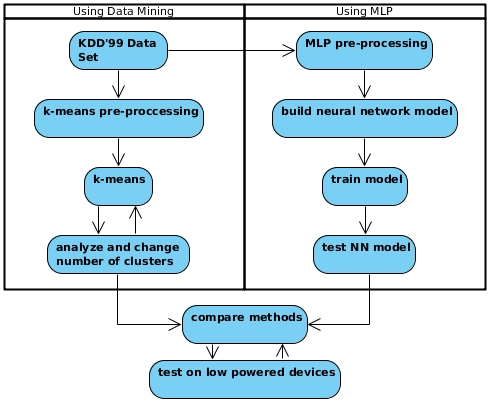
\includegraphics{methodology}

	\section{Time Line}
	\begin{itemize}
		\item 30 Jan 2018: Acquire and understand KDD'99 data-set
		\item 12 Feb 2018: Implement \cite{dm15} on KDD'99
		\item 28 Feb 2018: Implement \cite{mlp17} on KDD'99
		\item 07 Mar 2018: Analyze and compare the two on regular devices
		\item 20 Mar 2018: Test on low powered devices
		\item 15 Apr 2018: Scale down algorithms for low powered devices
		\item 01 May 2018: Re-run tests and understand pros and cons of scaling down
	\end{itemize}

	%References
	\bibliographystyle{IEEEtran}
	\bibliography{references}
	\end{document}
		  